\section{Findings}

%%%% Tasks
\begin{frame}{Conclusion}
\begin{columns}[c,onlytextwidth]
\begin{column}{0.7\textwidth}
\vspace{-1.8em}
\uncover<1->{
\begin{block}{Task 1}
Integrate both sources of information into a single formal lattice.
\end{block}
}
\uncover<2->{
    \begin{itemize}
        \item \ac{mlb} constraints, i.e., expert knowledge
        \item Case study: BankSearch dataset
        \begin{itemize}
            \item Trivial context from dataset
        \end{itemize}
    \end{itemize}
}
% \vspace{2.8em}
\uncover<3->{
\begin{block}{Task 2}
    Analyze the agreement of a data-driven formal lattice and an expert knowledge formal lattice.
\end{block}
}
\uncover<4->{
    \begin{itemize}
        \item Consistency and coherence lattice
        \item Case study: BankSearch dataset
    \end{itemize}
}
\end{column}
\begin{column}{0.3\textwidth}
\uncover<2->{
    \centering
    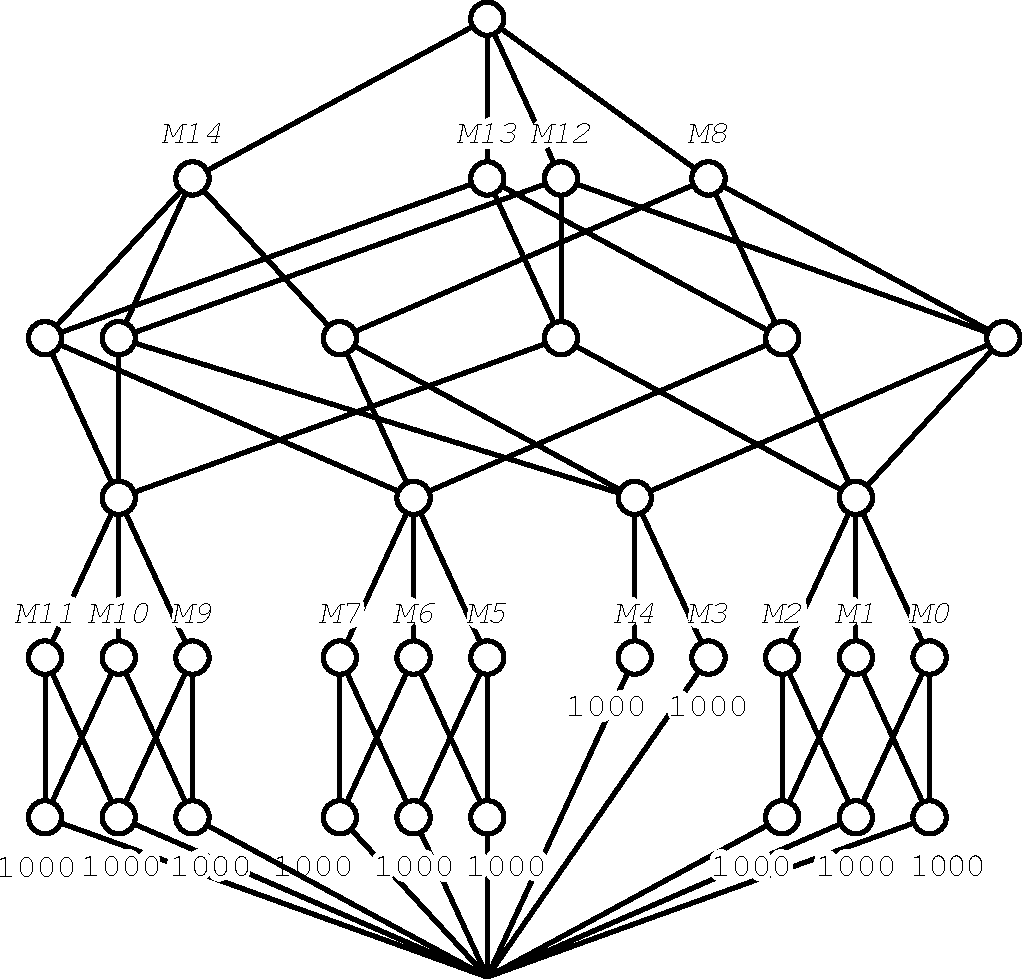
\includegraphics[width=\textwidth,height=0.35\textheight,keepaspectratio]{slides/figures/mlb_expanded.pdf}
}
\vspace{0.5em}
\uncover<4->{
\centering
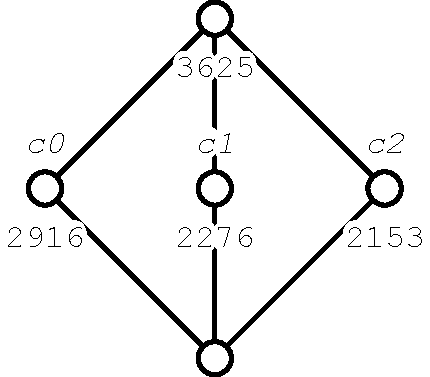
\includegraphics[width=\textwidth,height=0.45\textheight,keepaspectratio]{results/context_comparison/CONCEPT_SIM/coherence.pdf}
}
\end{column}
\end{columns}
\end{frame}










